\section{Información del entorno}

\subsection{Descripción del entorno}
El entorno operativo de PetShop Huellitas \& Snacks está conformado por los siguientes actores clave:
\begin{itemize}
    \item \textbf{Proveedores:} Distribuidoras mayoristas de alimentos premium nacionales y extranjeras, y fabricantes de accesorios y snacks.
    \item \textbf{Clientes:} Propietarios de mascotas domésticas, albergues de rescate animal y clínicas veterinarias minoristas del norte de Quito.
    \item \textbf{Competencia:} Grandes supermercados locales, almacenes agropecuarios y otras tiendas online que comercializan alimento para mascotas.
    \item \textbf{Estado:} El Servicio de Rentas Internas (SRI) que norma la emisión de facturación electrónica y entidades de control de registros sanitarios.
    \item \textbf{Comunidad:} Fundaciones locales de protección de mascotas, dueños de mascotas de la zona residencial y vecinos del local.
\end{itemize}

\subsection{Entidades}
\begin{enumerate}
    \item \textbf{Cliente (Actor Externo):} Interactúa con el sistema para consultar productos, realizar compras y recibir notificaciones y comprobantes electrónicos.
    \item \textbf{Administrador / Vendedor (Actor Interno):} Administra el catálogo de productos, visualiza reportes de stock, aprueba pedidos y despacha compras.
    \item \textbf{Proveedor (Actor Externo):} Sistema o persona que recibe solicitudes automáticas de reabastecimiento generadas por el sistema.
    \item \textbf{Pasarela de Pagos (Sistema Externo):} Entidad bancaria o pasarela transaccional externa encargada de validar los pagos electrónicos de los pedidos.
    \item \textbf{Facturación SRI (Sistema Externo):} Servicio del Estado que valida, autoriza y firma la emisión de comprobantes electrónicos del local.
\end{enumerate}

\subsection{Modelo de Contexto}
El diagrama de contexto define la frontera del sistema ``PetFood-Manager'', determinando los flujos de datos entrantes y salientes entre la aplicación central y las entidades externas definidas previamente.
\begin{figure}[H]
    \centering
    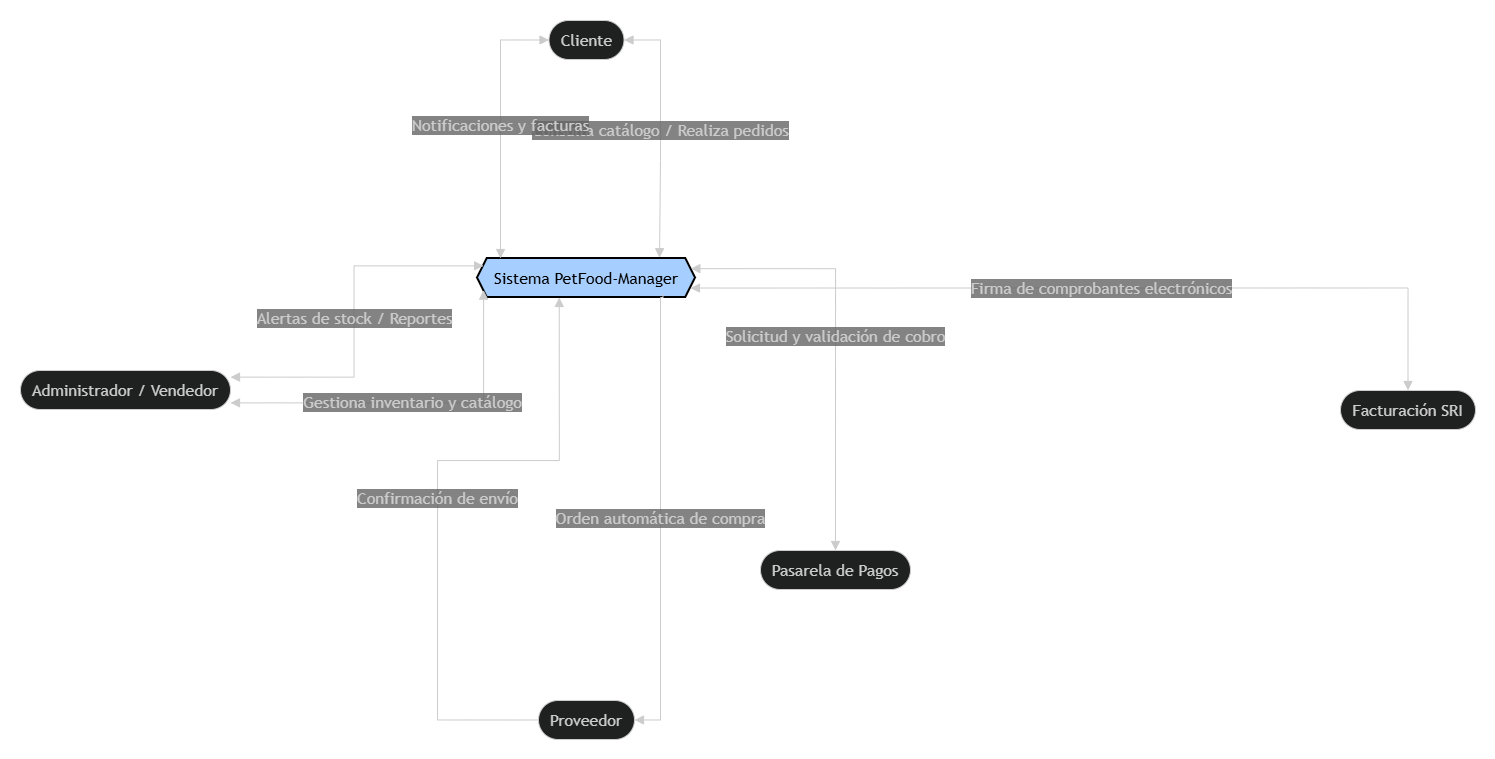
\includegraphics[width=0.60\textwidth]{Images/modeloContexto.png}
    \caption{Diagrama de Modelo de Contexto}
    \label{fig:modelo_contexto}
\end{figure}

\subsection{Diagrama de Flujo de Datos Nivel 0}
El DFD Nivel 0 subdivide el comportamiento del sistema en tres procesos transaccionales centrales que interactúan de forma directa con los almacenes de datos de la tienda.
\begin{figure}[H]
    \centering
    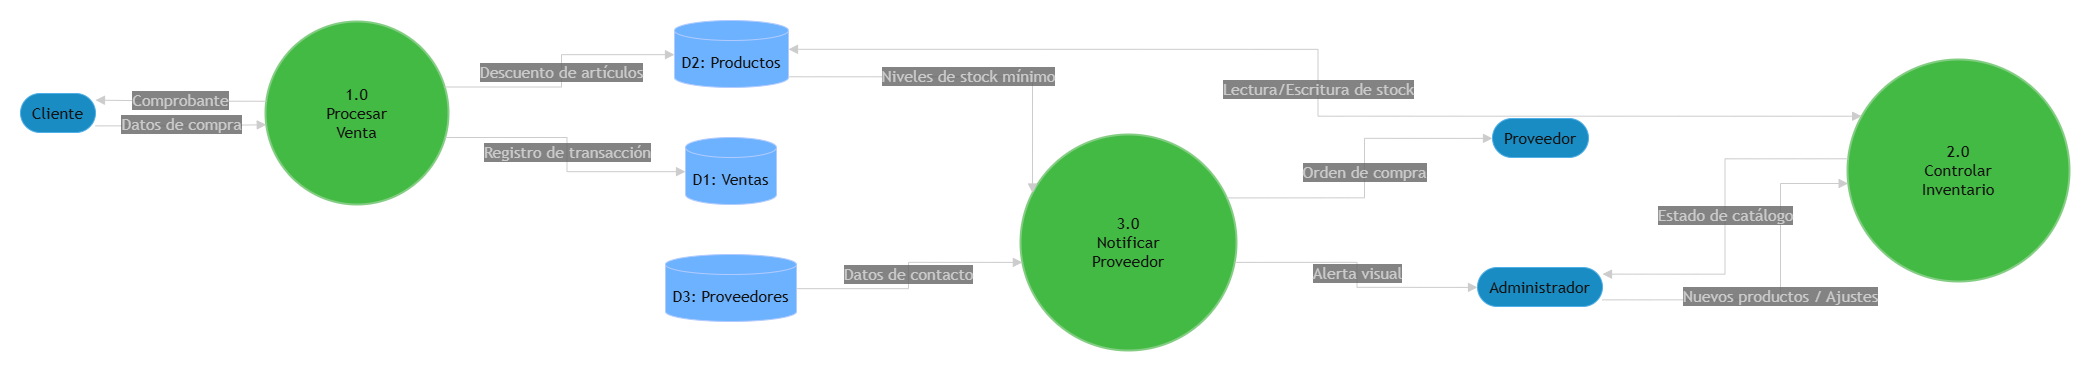
\includegraphics[width=0.60\textwidth]{Images/diagramaFlujo.png}
    \caption{Diagrama de Flujo de Datos (DFD) Nivel 0}
    \label{fig:dfd_nivel_0}
\end{figure}